Un computer, classico o quantistico che sia, ha lo scopo di gestire e manipolare informazioni; le quali come unità di misura fondamentale hanno il \underline{BIT} (dall'inglese Binary digIT).\\
Nei computer quantistici viene però usata una variante denominata \underline{QUBIT} (QUantum BIT), la quale ha comportamenti di tipo quantistico.
\section{Bit}
\subsection{Teoria}
Un bit, sumbolo \textit{b}, può assumere solamente 2 valori: \{\textit{0}, \textit{1}\}, ma è sufficiente per svolgere ogni processo e rappresentare ogni tipo di informazione, qualche esempio:
\begin{enumerate}
\item I numeri (in formato binario) si possono ottenere direttamente con una sequenza di bit, e si possono convertire facilmente in decimale per facilitare la comprensione umana:\\
\textsc{0 = 0}; \textsc{1 = 1}; \textsc{10 = 2}; \textsc{1011 = 11}...
\item Le stringhe (parole, frasi ecc...) non sono altro che insieme di caratteri. Questi ultimi sono rappresentati come numeri e quindi come insiemi di bit; le tabelle di conversione più famose e usate sono la \textit{ASCII} e la \textit{UNICODE}; ad esempio in \textit{ASCII}:\\
97 = \textit{a} ; 125 = \textit{\}} ; 32 = [\textit{Space}]\\
\item Anche le immagini non sono altro che insiemi di numeri; esse sono infatti formate da pixel, ognuno dei quali è composto da tre numeri: componente rossa, componente verde e componente blu; sono difatti matrici tridimensionali. Ovviamente più pixel ci sono più l'immagine sarà di alta qualità, ma comunque se ingrandita ad un certo punto si nota come sia composta da piccoli quadrati. Esiste però un modo di evitarlo per alcune immagini definite e ben conosciute (ad esempio i caratteri) ed è quello di descrivere l'immagine tramite una funzione che definisce un numero definito di pixel (in modo che non siano visibili) indipendentemente dallo zoom.
\end{enumerate}
In quanto unità molto piccola si parla molto più spesso dei multipli dei bit, piuttosto che di essi stessi; i quali però seguono regole un po' particolari rispetto alle grandezze fisiche:\\
Il \textit{Byte}, simbolo \textit{B} è composto da 8 bit e quindi può contenere $2^8 = 256$ diverse combinazioni e quindi rappresentare numeri tra 0 e 255.\\
I prefissi utilizzati sono il \textit{k/kilo-}, il \textit{M/mega-}, il \textit{G/giga-} e il \textit{T/tera-}; ma invece di corrispondere (rispetto al precedente) ad un fattore 1000 come accade solitamente (ad esempio un kilogrammo corrisponde a 1000 grammi) corrispondono ad un fattore 1024; per potersi legare alle potenze di due ($2^{10}$=1024); ad esempio:\\
1 kB = 1024 B; \ 1 MB = 1024 kB = $2^{28}$ bit.
\subsection{Hardware}
L'informazione (i bit) è implementata nella realtà in moltissimi modi che si sono evoluti nell'ultimo secolo; tra i più famosi:
\begin{enumerate}
\item I floppy disk furono tra le più famose unità di memoria negli anni 70 e 80 seppur oggi sono praticamente scomparsi e quasi dimenticati. Erano formati da un disco di materiale ferromagnetico diviso in zone ognuna delle quali per rappresentare i due stati \textit{0} o \textit{1} veniva magnetizzata con il polo nord verso l'alto oppure verso il basso; vantaggio principale era il fatto che poteva essere letto e riscritto un numero teoricamente infinito di volte; però poteva essere facilmente rovinato da campi magnetici ambientali non prevedibili; per di più non permettevano di accedere ad una determinata informazione in modo istantaneo, ma andava ricercata partendo dall'inizio (come accadeva anche per le vecchie videocassette). La capacità media si aggirava intorno ai pochi megabyte.
\item I CD i DVD e i blu-ray sono usati ancora oggi pur molto meno di una decina di anni fa e sono composti da un disco ottico. Cioè per rappresentare 0 o 1 ogni zona può essere bruciata o meno in modo che rifletta oppure no. Le differenze tra loro risiedono soprattutto nella capacità: i CD sono circa 700 MB; i DVD 4 GB e i blu-ray 25GB. Gli hard disk usati nei computer oggi non sono altro che tanti dischi.
\item La memoria flash è la più utilizzata attualmente; ne fanno uso le chiavette USB, le SD card e gli SSD. Ogni bit è composto da un insieme di 5 transistor e questa è la tecnologia migliore; consuma meno, è più affidabile e può avere maggiore capacità. Il problema principale è che la memoria flash non è persistente, ma nel giro di 10-20 anni può perdere informazione. Costa anche un po' di più ma data la \textit{Legge di Moore} il costo tende a scendere. La Legge di Moore è una legge empirica che afferma che circa ogni due anni è possibile produrre transistor di dimensioni dimezzate; il che permette capacità maggiori a costo inferiore. La capacità della memoria flash è infatti molto variabile ed esistono dispositivi di ogni taglia, ma gli SSD più capienti in genere sono dell'ordine del TB.
\item Una menzione va fatta anche alla RAM; essa somiglia alla memoria flash, ma è molto più veloce; è possibile accedere a qualsiasi informazione nell'ordine dei nanosecondi, nei computer attuali ne sono presenti diversi GB. La nota negativa (a parte il costo) è il fatto che la memoria non è persistente e quindi quando cessa l'alimentazione ogni dato viene perso. Il suo uso è quindi quello di permettere di lavorare in tempo reale su informazioni che poi verranno copiate (=salvate) su altra tipo di memoria.
\end{enumerate}
\section{Qubit}
\subsection{Teoria}
Similarmente al bit anche i qubit possono assumere solamente due valori: \{\textit{0, 1}\} però non obbligatoriamente come \textit{autovalori}.
Un qubit è quindi un sistema quantico che può assumere due livelli energitici: \{$\ket{0}$, $\ket{1}$\} ove $\ket{0}$ viene spesso definito \textit{terra} in quanto più basso energeticamente.  Assieme formano quello che si chiama \textit{standard basis vector}; un elemento di algebra lineare. Come tutti i vettori essi hanno \textit{direzione, verso e modulo}; ma potendo avere anche coefficienti complessi i qubit dispongono anche di una \textit{fase}. Per rappresentare ogni possibile superposizione di un qubit viene usata la dicitura $\alpha\ket{0} + \beta\ket{1}$ ove \{$\alpha,\beta \in \mathbb{C}$\}. Con $|\alpha|^2$ si ottiene la probabilità di ottenere il valore 0 e $|\beta|^2$ quella del valore 1; essendo poi volori di probabilità $|\alpha|^2 + |\beta|^2 = 1$ sempre.\\
Volendo semplificare il più possibile in questa tesina si cercherà di evitare terminologie matematiche di algebra lineare; per i qubit useremo sempre quindi una rappresentazione grafica, detta \underline{BLOCH SPHERE}; ciè una sfera di raggio 1 in cui ogni punto sulla sua superficie rappresenta un qubit:\\
\begin{center}
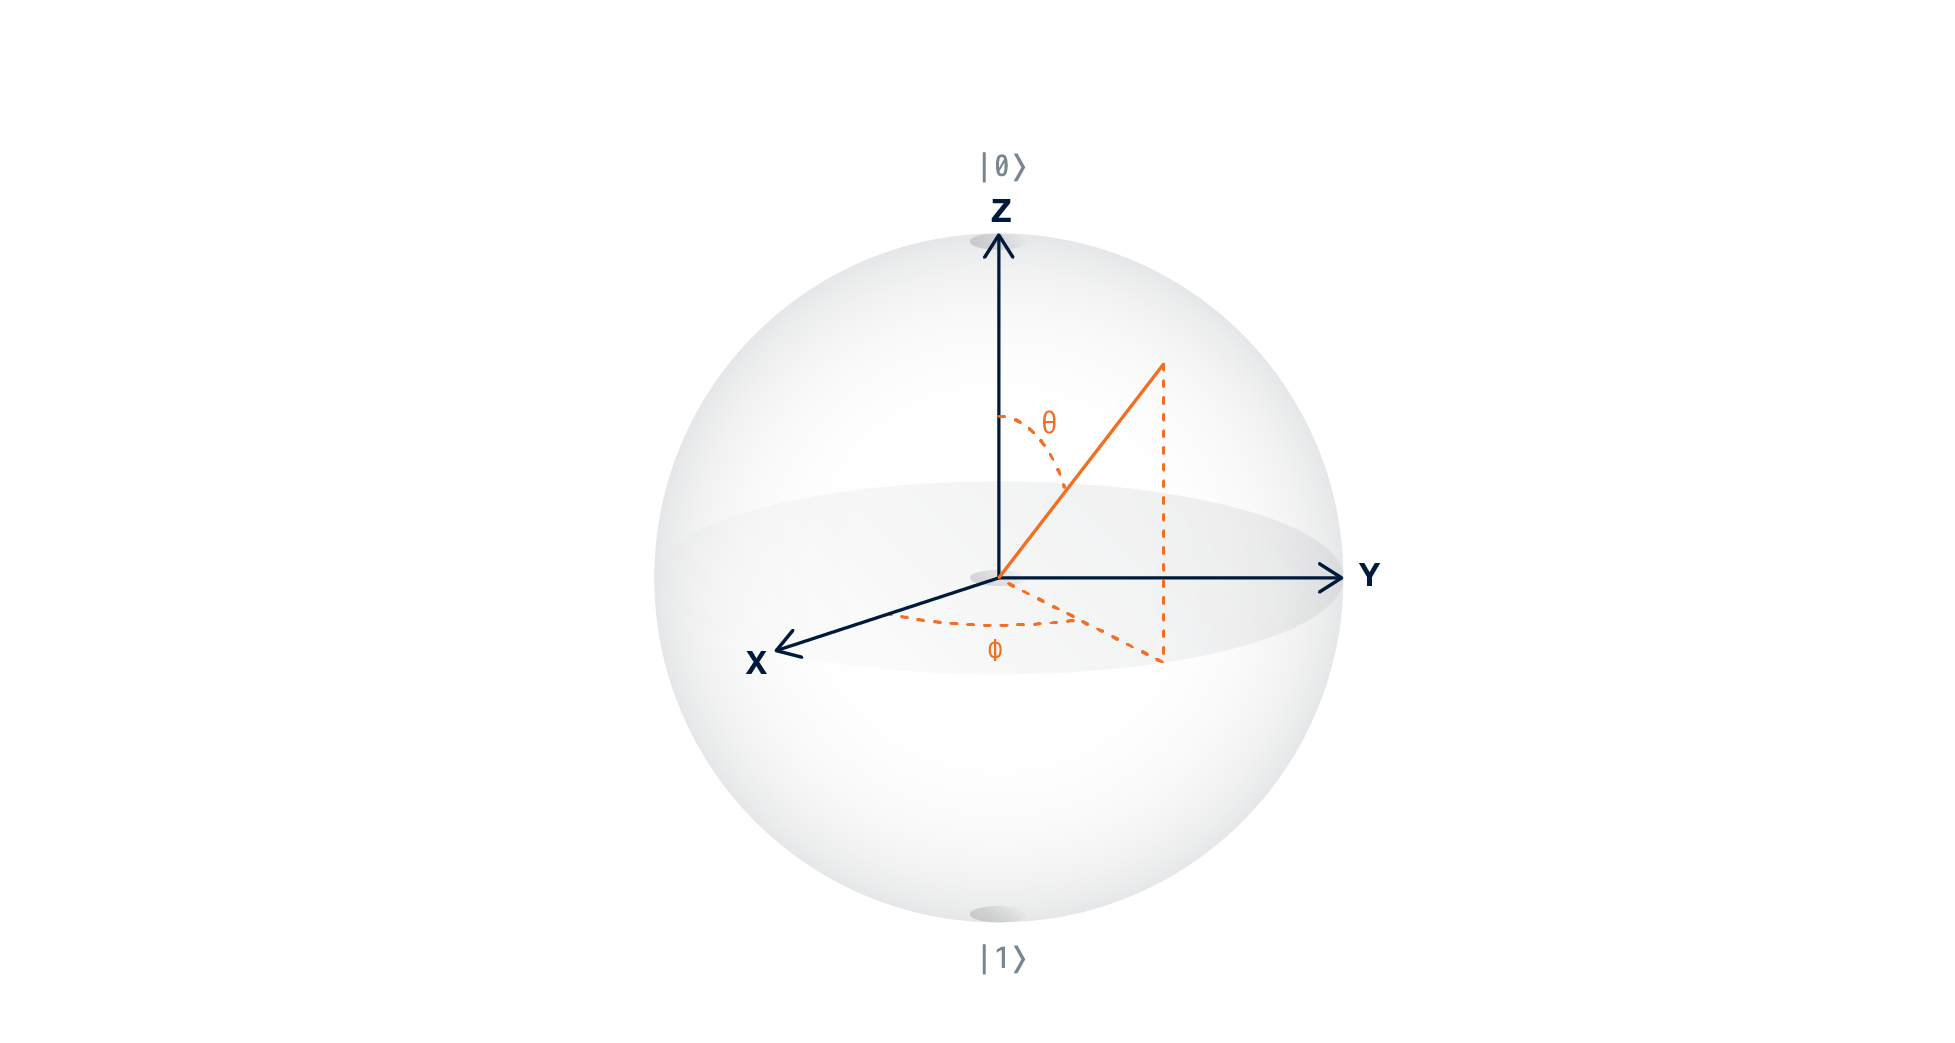
\includegraphics[scale=0.5]{exampleBlochSphere}
\end{center}
I punti allineati all'asse Z rappresentano gli autostati; in cima alla sfera il valore è $\ket{0}$; in fondo $\ket{1}$. In qualsiasi altro punto si ha superposizione; in particolare le rotazioni intorno all'asse Z (angolo rappresentano la fase. L'angolo $\theta$ modifica quindi le probabilità di ottenere i due valori \{\textit{0, 1}\}, ma non l'angolo $\phi$ (fase); difatti la fase è un'informazione che si va a perdere quando si fa il quadrato del modulo di $\alpha$ e $\beta$. La fase però non è inutile in quanto applicando trasformazioni (come si vedrà nel capitolo successivo) al qubit determinerà risultati diversi anche in $|\alpha|^2$ e $|\beta|^2$
\subsection{Hardware}
La costruzione fisica dei qubit è al giorno d'oggi uno dei problemi maggiori in quanto i fenomeni quantistici si presentano solo in condizioni particolari, in genere nel microscopico, e quindi molto instabili e difficilmente controllabili.\\
Le soluzioni proposte e adottate sono molteplici, ma la più famosa adottata da D-WAVE e da GOOGLE (chiamata SQUID) è quella di utilizzare un particolare metallo chiamato Niobio (\textit{Nb}), numero 41 sulla tavola periodica.
La scelta è data dal fatto che viene sfruttato il campo magnetico generato quando è in stato di superconduttore e tra gli elementi puri il \textit{Nb} è quello che diventa tale alla temperatura più alta (9,25K) e genera uno dei campi magnetici maggiori.\\
\begin{center}
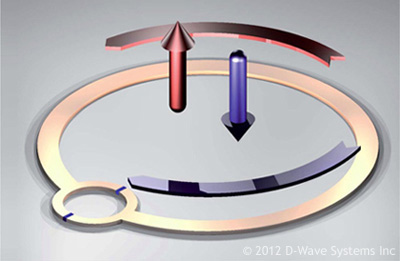
\includegraphics[scale=1.5]{niobiumQubit}
\end{center} 
Come si vede dall'immagine il campo generato può avere due versi opposti (frecce blu e rosse ed esso si comporta in modo quantistico e il verso è descritto da un vettore di stato che non assume obbligatoriamente autovalori quindi uno può rappresentare $\ket{0}$ e l'altro $\ket{1}$.\\
Ad oggi si è arrivati a produrre anche chip con anche una cinquantina di qubit, veramente pochi a confronto dei milioni necessari a rendere i computer quantistici utili a livelllo commerciale, quindi altri modi di creare qubit sono in fase di ricerca (principalmente basati su fotoni e elettroni), ma lo stadio è molto precoce.
